\documentclass[12pt]{article}

\usepackage{setspace}
\usepackage{fancyvrb}
\usepackage{graphicx}
\usepackage{geometry}
\usepackage{multirow}
\usepackage{array}
\usepackage{color}
\usepackage{hyperref}
\setlength{\parindent}{4em}
\geometry{letterpaper, portrait, margin = 1in}

\newcommand\tab[1][1cm]{\hspace*{#1}}
\renewcommand\thesection{\arabic{section}}
\renewcommand\thesubsection{\thesection.\arabic{subsection}}

%%%Title Page%%%
\title{
	\begin{center}
		
\includegraphics[scale=0.5]{uga.png}\\
 	\end{center}
 	Project 04
	\bigbreak Design Notebook
}
\author{\textbf{Zachary Davis}}

\date{\today}
%%%%%%%%%%%%%%%%%

\begin{document}
	
	%%%Title Page%%%
	\vspace{\fill}
	\maketitle
	\vspace{\fill}

	%%%Table of Contents%%%
	\newpage
	\setstretch{2.5} % for custom spacing
	\tableofcontents
	\setstretch{1} % for custom spacing
	\newpage

\section{Problem Statement}
	\paragraph*{}
		Day-to-day operation for nurses and doctors at Children’s Healthcare of Atlanta is very
		important and worrying about the location and state of their equipment should not be high on that list.\\
		\tab Employees of the hospital should be able to see if a ventilator is in use, needs maintenance or repair, and where it is in the hospital all in a way that is easy and efficient, so not to distract them from there more important tasks. The added equipment that gives this functionality should be small, unnoticeable, and removable so that rented ventilators are not permanently modified. It should also be very simple. The point of this modification is to make equipment use more ubiquitous across the hospital and it should not create more issues than it solves.\\
		\tab However, the current equipment management at Children’s is inefficient and wastes the hospitals time and resources, not to mention the patients. By not having this information at employee’s fingertips we waste their time and efforts searching for equipment like ventilators rather than treating their patients. Because of this, the patients of Children’s will have a less than perfect and optimized experience and potentially decrease the company image.\\
		\tab By adding a simple device that can use wireless and Bluetooth signal frequencies generated in the hospital we can triangulate the position of a ventilator to within a room. We can also state its current maintenance and repair status as well as whether it is in use. This means that in a matter of minute any employee can know where the nearest ventilator is.\\
		\tab For a financial budget, we as a team are still somewhat unsure but we do know we will need a Raspberry pi zero w which includes on board WIFI and Bluetooth and costs roughly twenty-five dollars on Amazon, an enclosure of sort that could possibly be created using a 3D printer or using the one included with the device, and then some RFID tags that will cost around ten dollars for a pack on Amazon as well. So as of right now we are looking at a budget of upwards of \$40.
		
		\begin{itemize}
			\item We met with our mentor, WenZhan Song in his office on September 1st, 2017.\\
			\item We held a conference call with Jocelyn Grunwell and Pradip Kamat on September 11th, 2017, but due to the inclement weather Dr. Kamat was not on the call.\\
		\end{itemize}

\section{Requirements}
	\begin{enumerate}
		\item Works on a 36 room, U-shaped floor of the hospital
		\item Locates accurately to each room on the floor
		\item Portable and removable system (for swapping out rented equipment)
		\item Shows whether the equipment is in use or available for use (LED light)
		\item Displays if equipment potentially needs maintenance (maintenance LED light comes on after a few months of use) 
		\item Application available to easily view equipment on iOS
	\end{enumerate}

\section{Contact w/ Clients}
	\begin{center}
		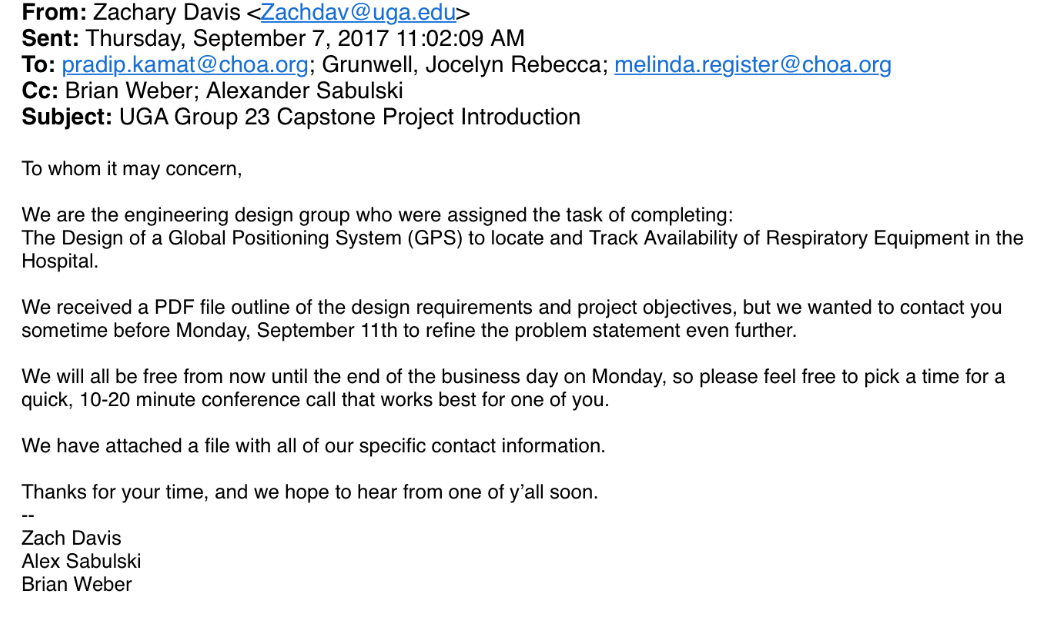
\includegraphics[scale=0.8]{1.png}\\
		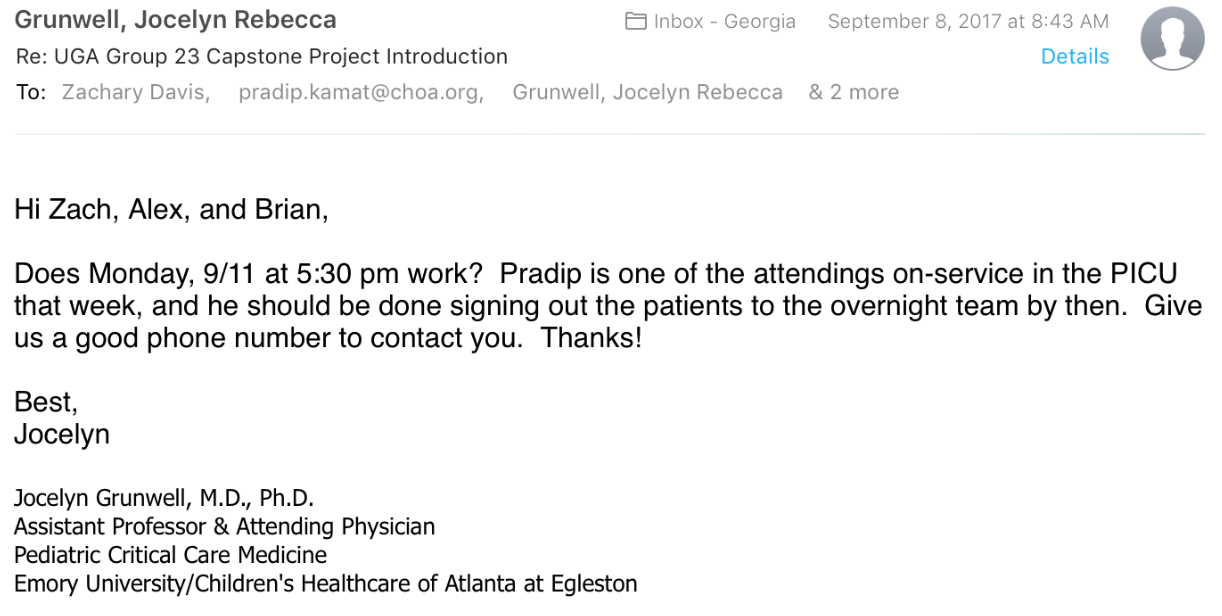
\includegraphics[scale=0.8]{2.png}\\
		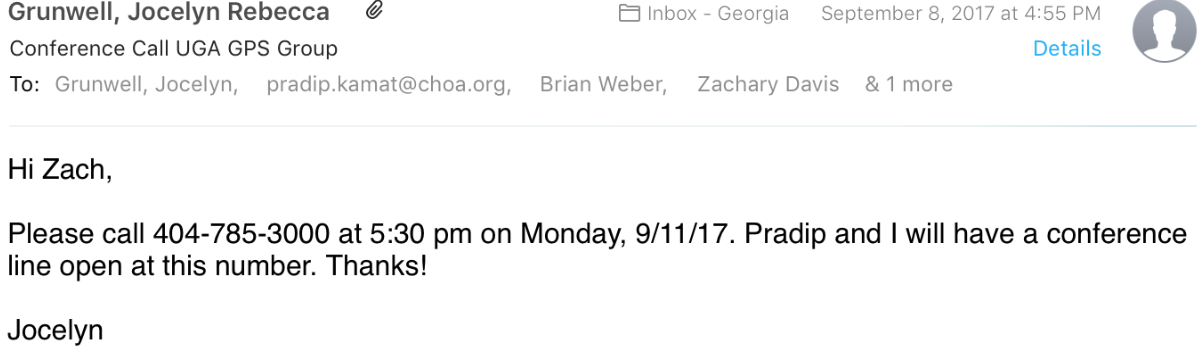
\includegraphics[scale=0.8]{3.png}\\
		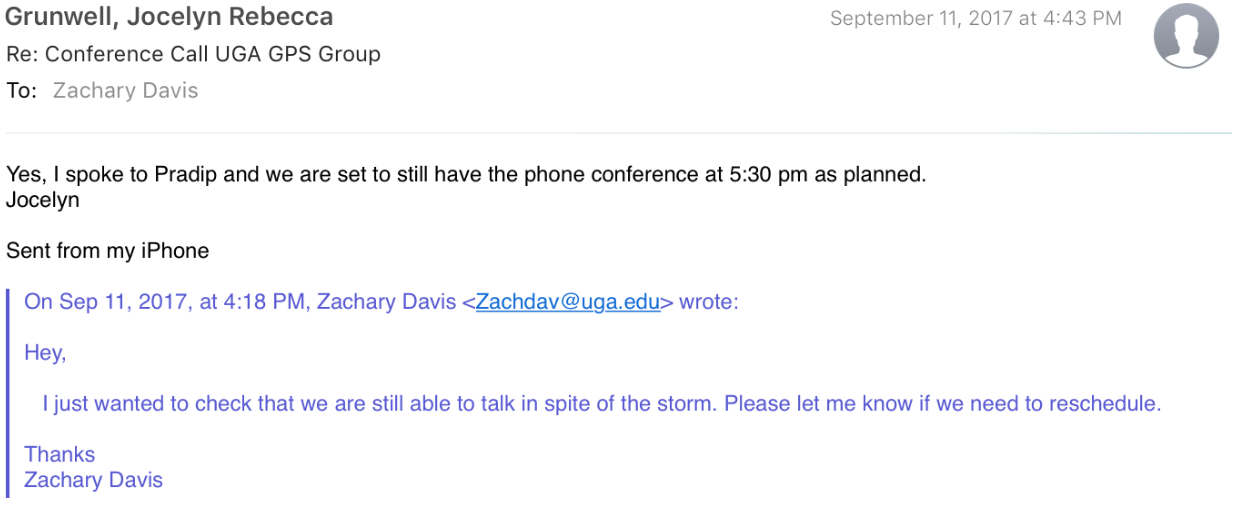
\includegraphics[scale=0.8]{4.png}\\
		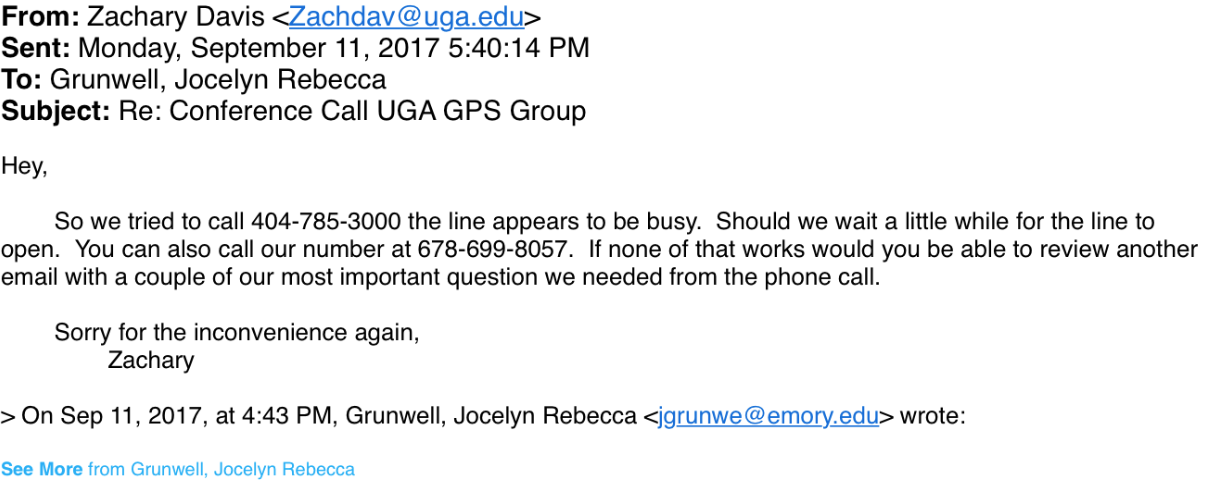
\includegraphics[scale=0.8]{5.png}\\
		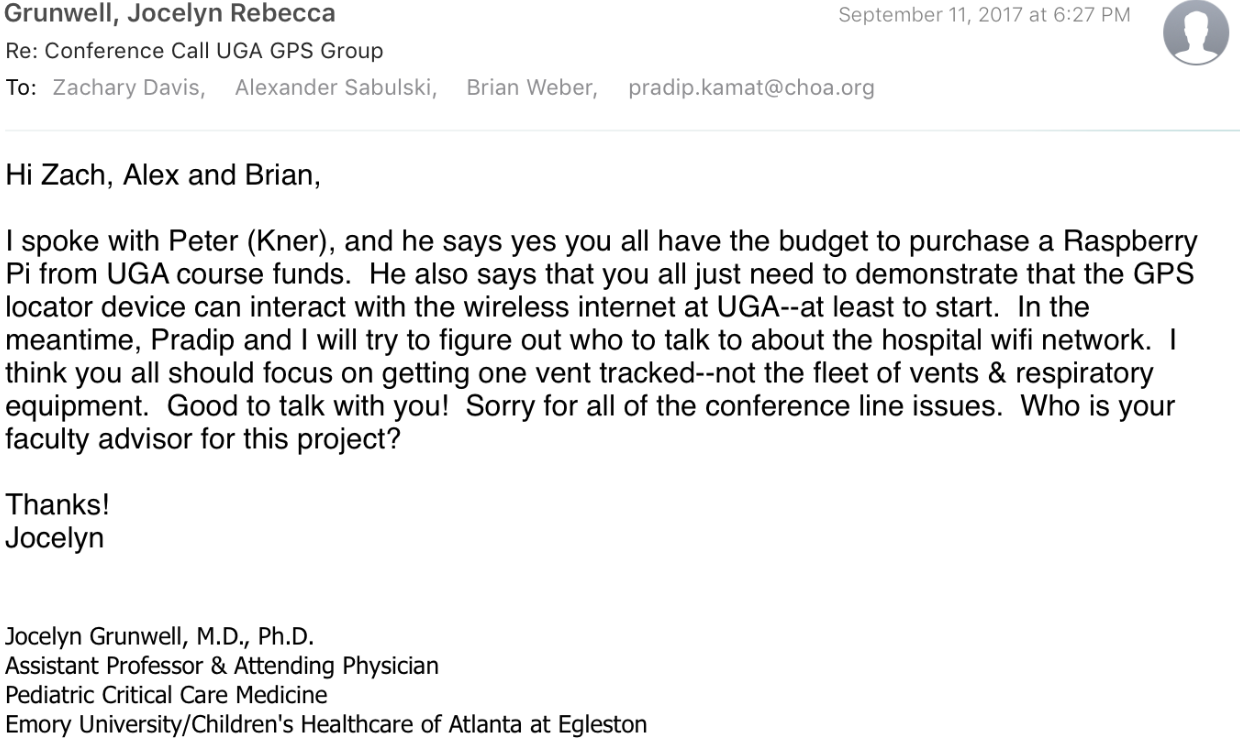
\includegraphics[scale=0.8]{6.png}\\
		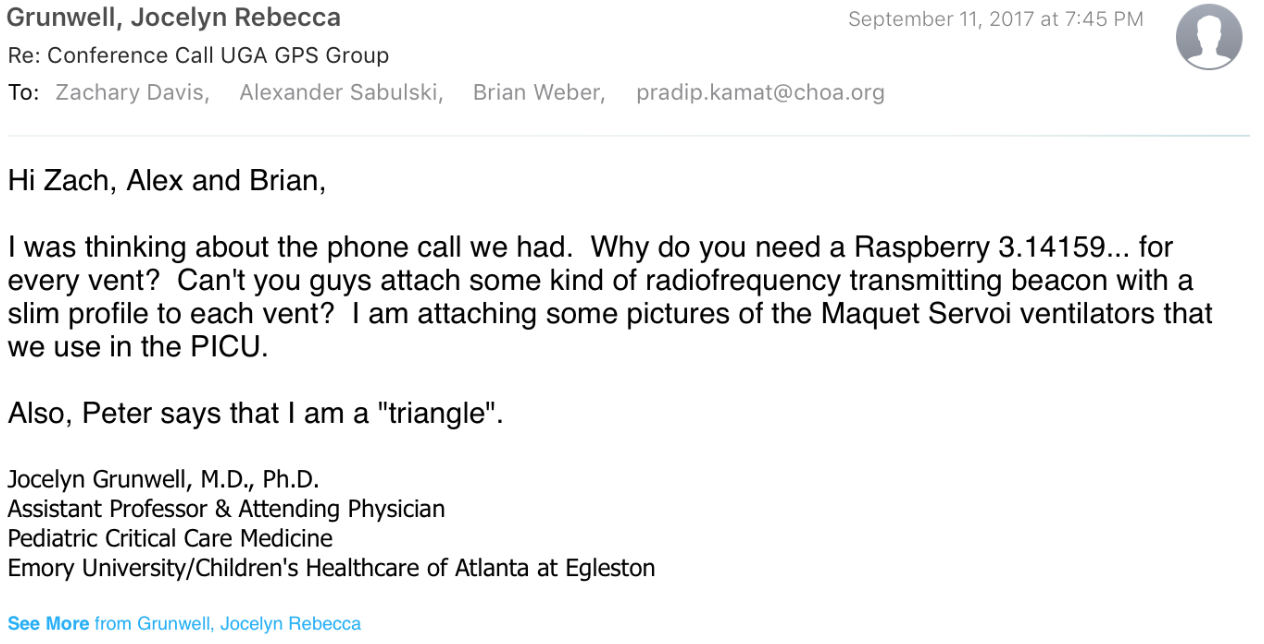
\includegraphics[scale=0.8]{7.png}\\
		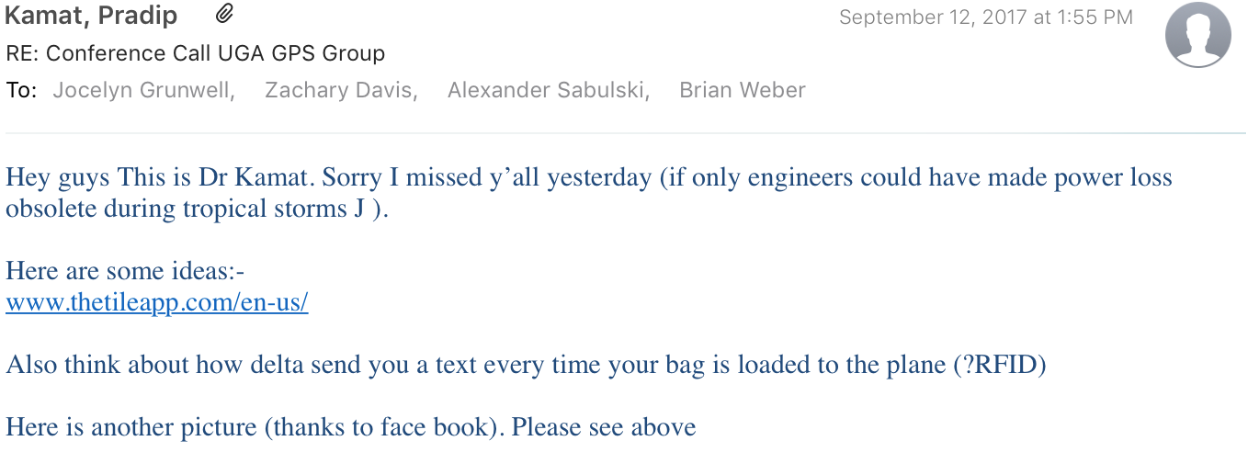
\includegraphics[scale=0.8]{8.png}\\
		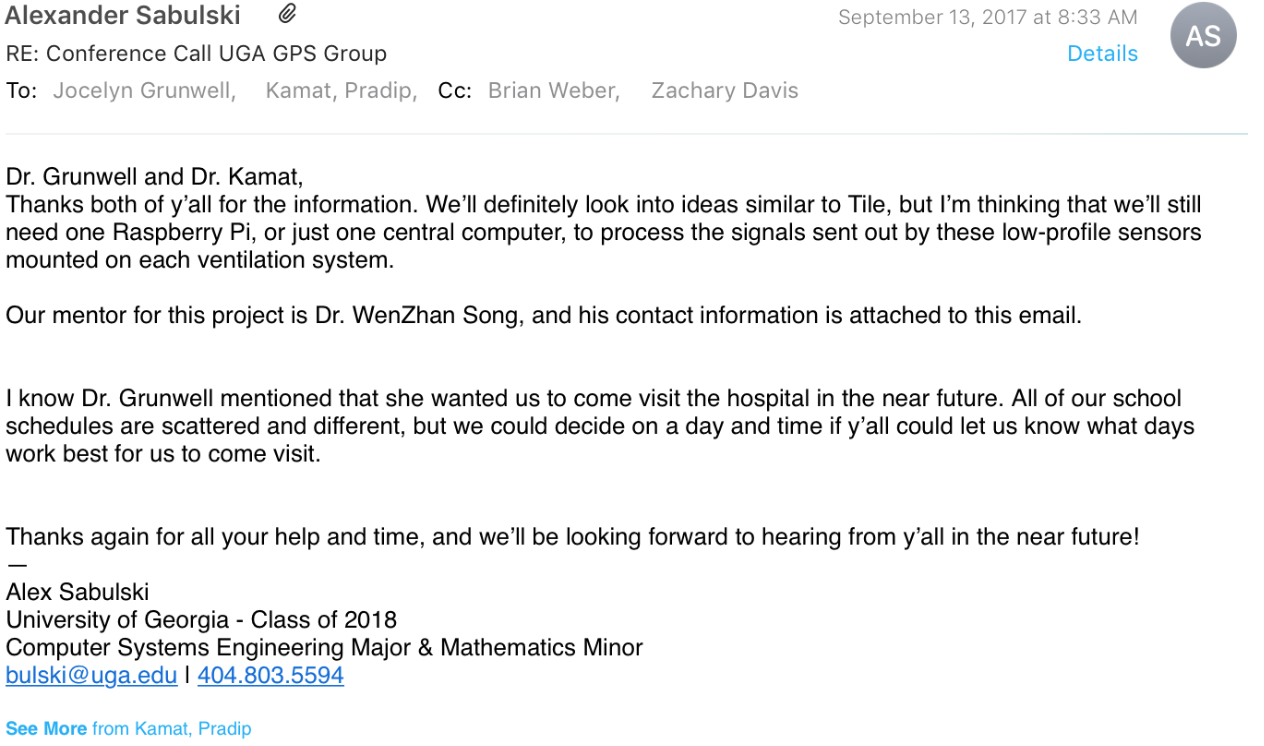
\includegraphics[scale=0.8]{9.png}\\
		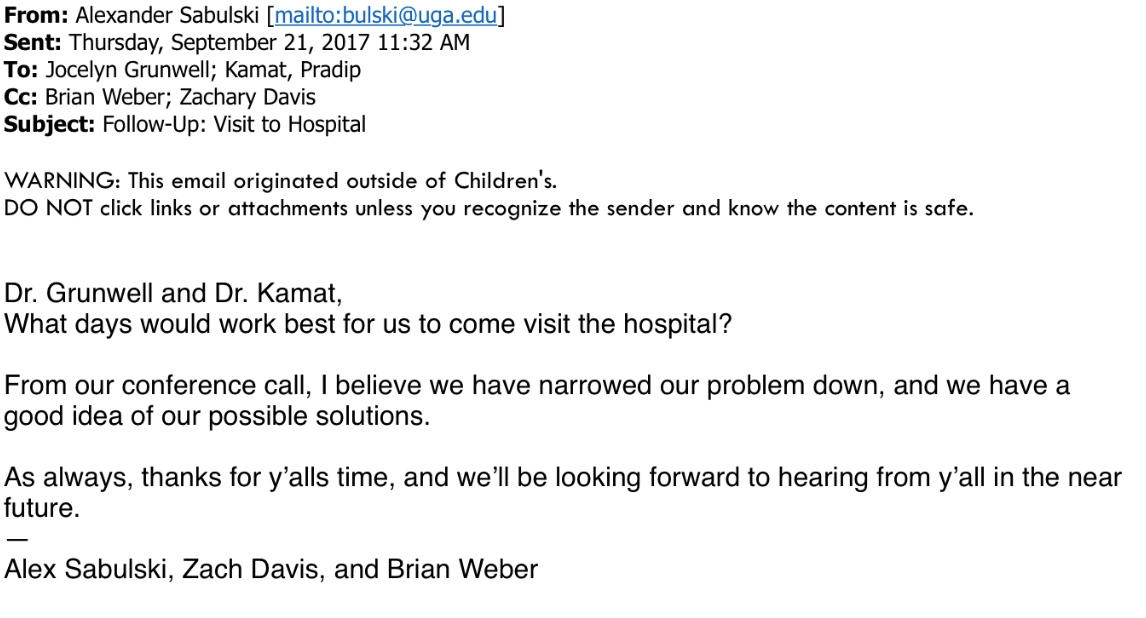
\includegraphics[scale=0.8]{10.png}\\
		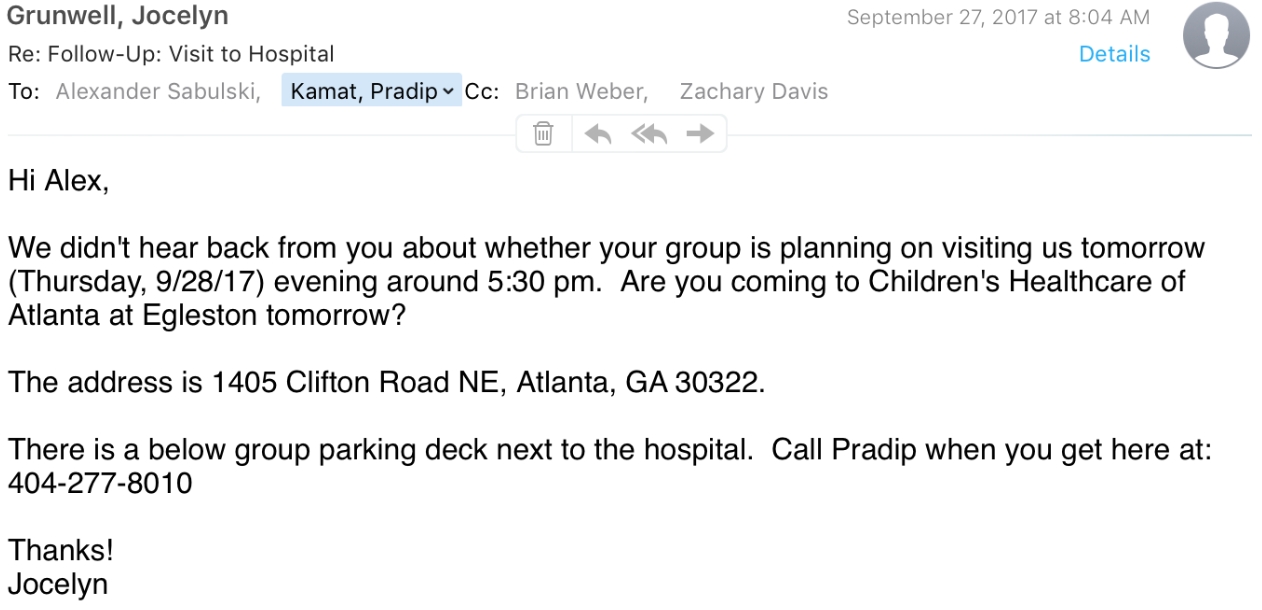
\includegraphics[scale=0.8]{12.png}\\
		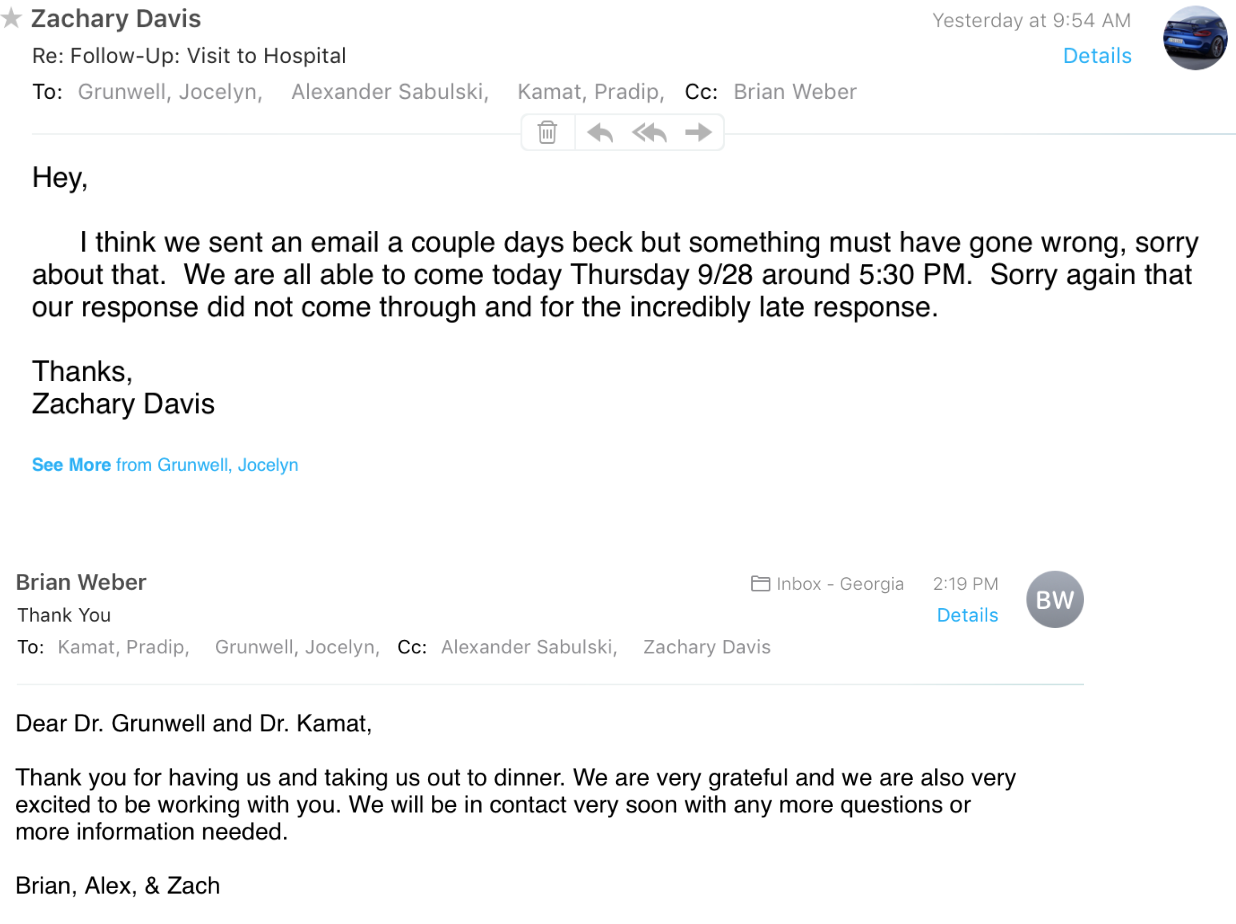
\includegraphics[scale=0.8]{13.png}\\
 	\end{center}

 \section{Visiting the Hospital}
 	\begin{center}
		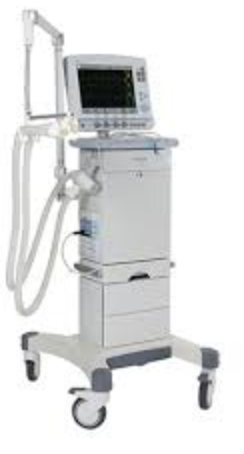
\includegraphics[scale=0.8]{h1.png}\\
		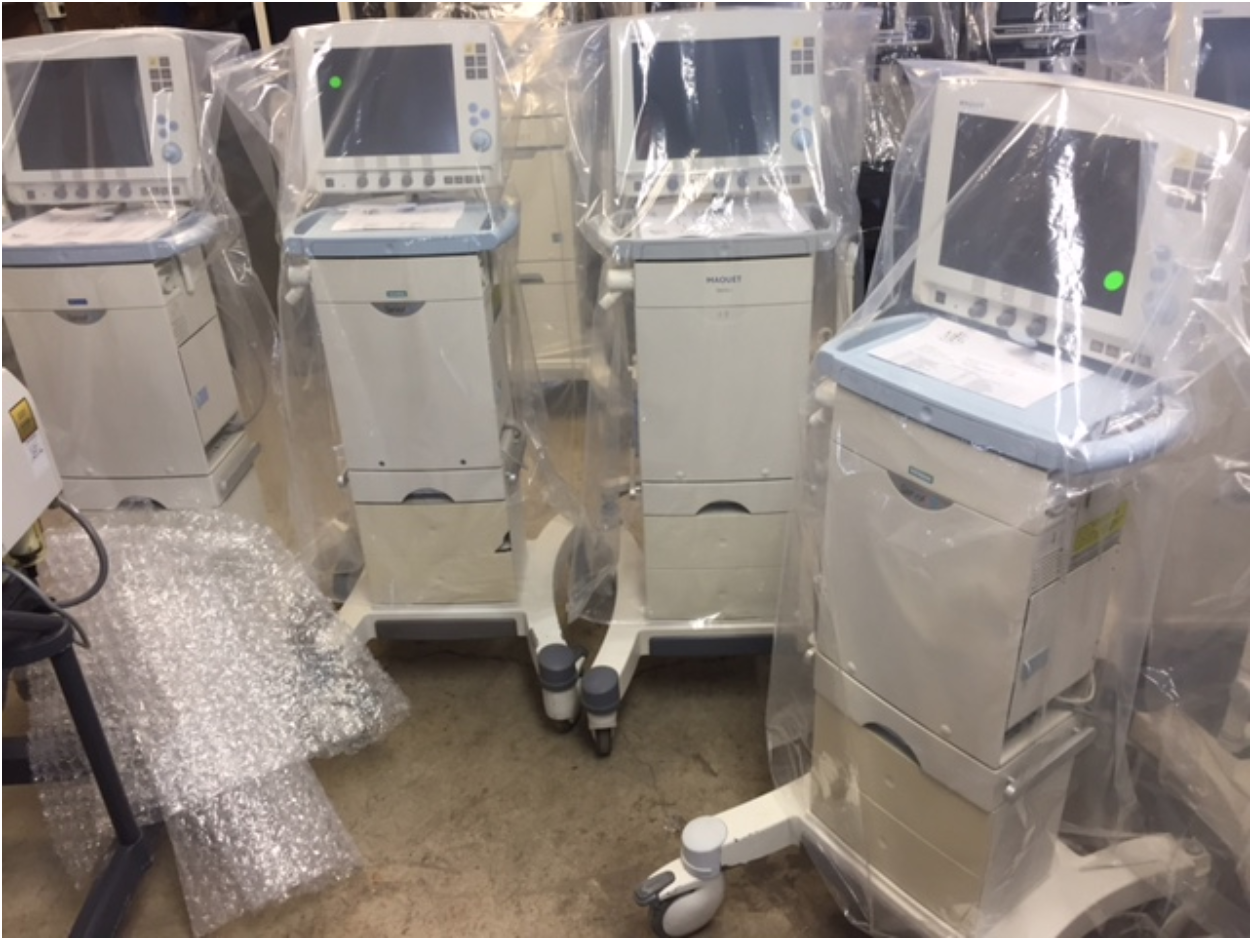
\includegraphics[scale=0.75]{h2.png}\\
		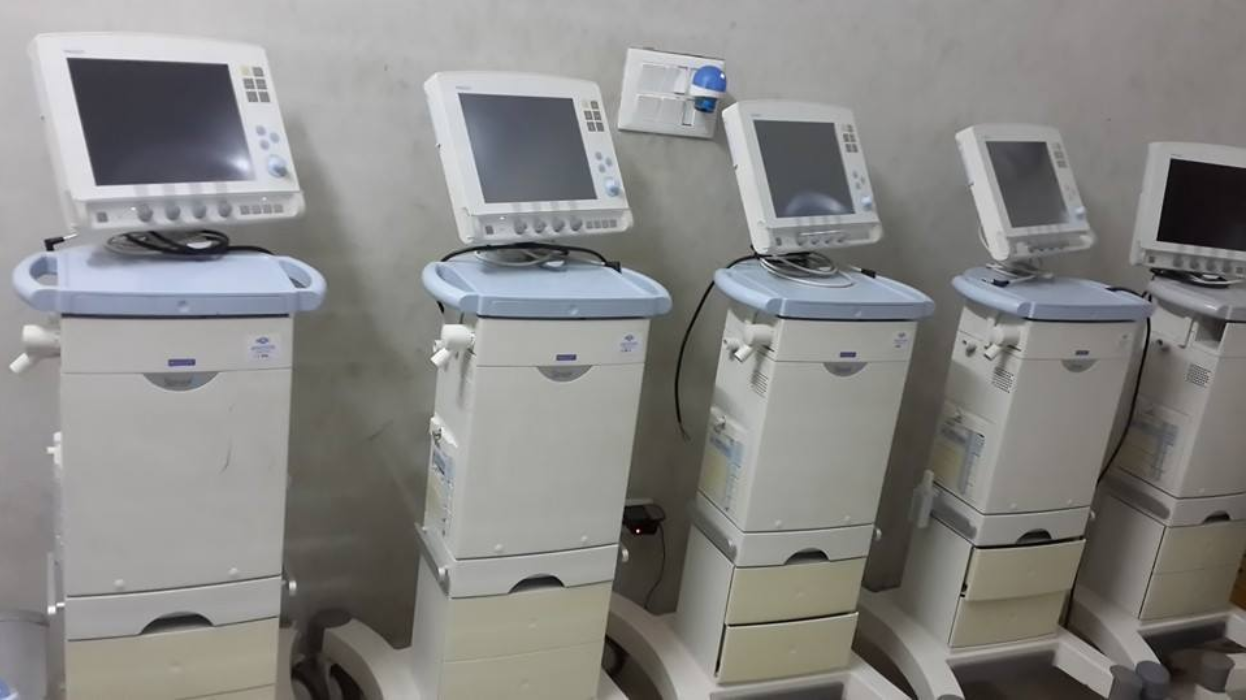
\includegraphics[scale=0.75]{h3.png}\\
	\end{center}

\section{Overall Plans}
	\subsection{Old Plan}
		\begin{center}
			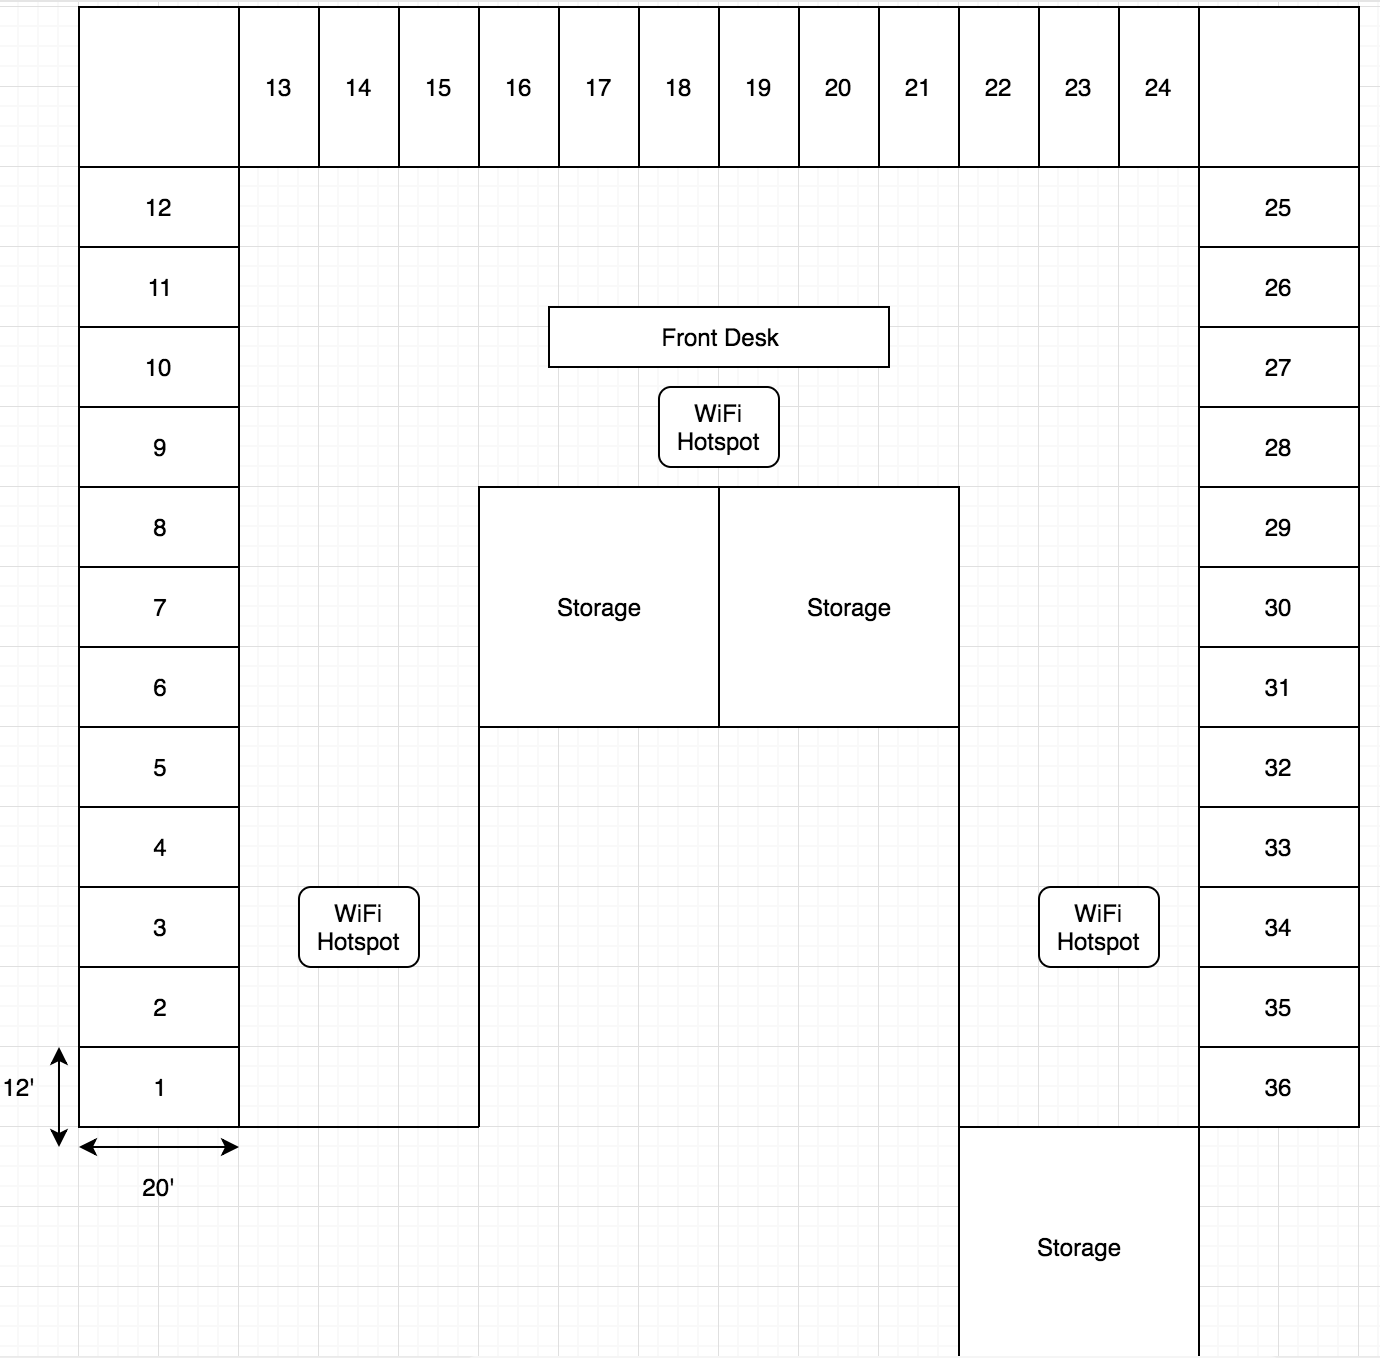
\includegraphics[scale=0.6]{op.png}\\
		\end{center}

	\subsection{New Plan}
		\begin{center}
			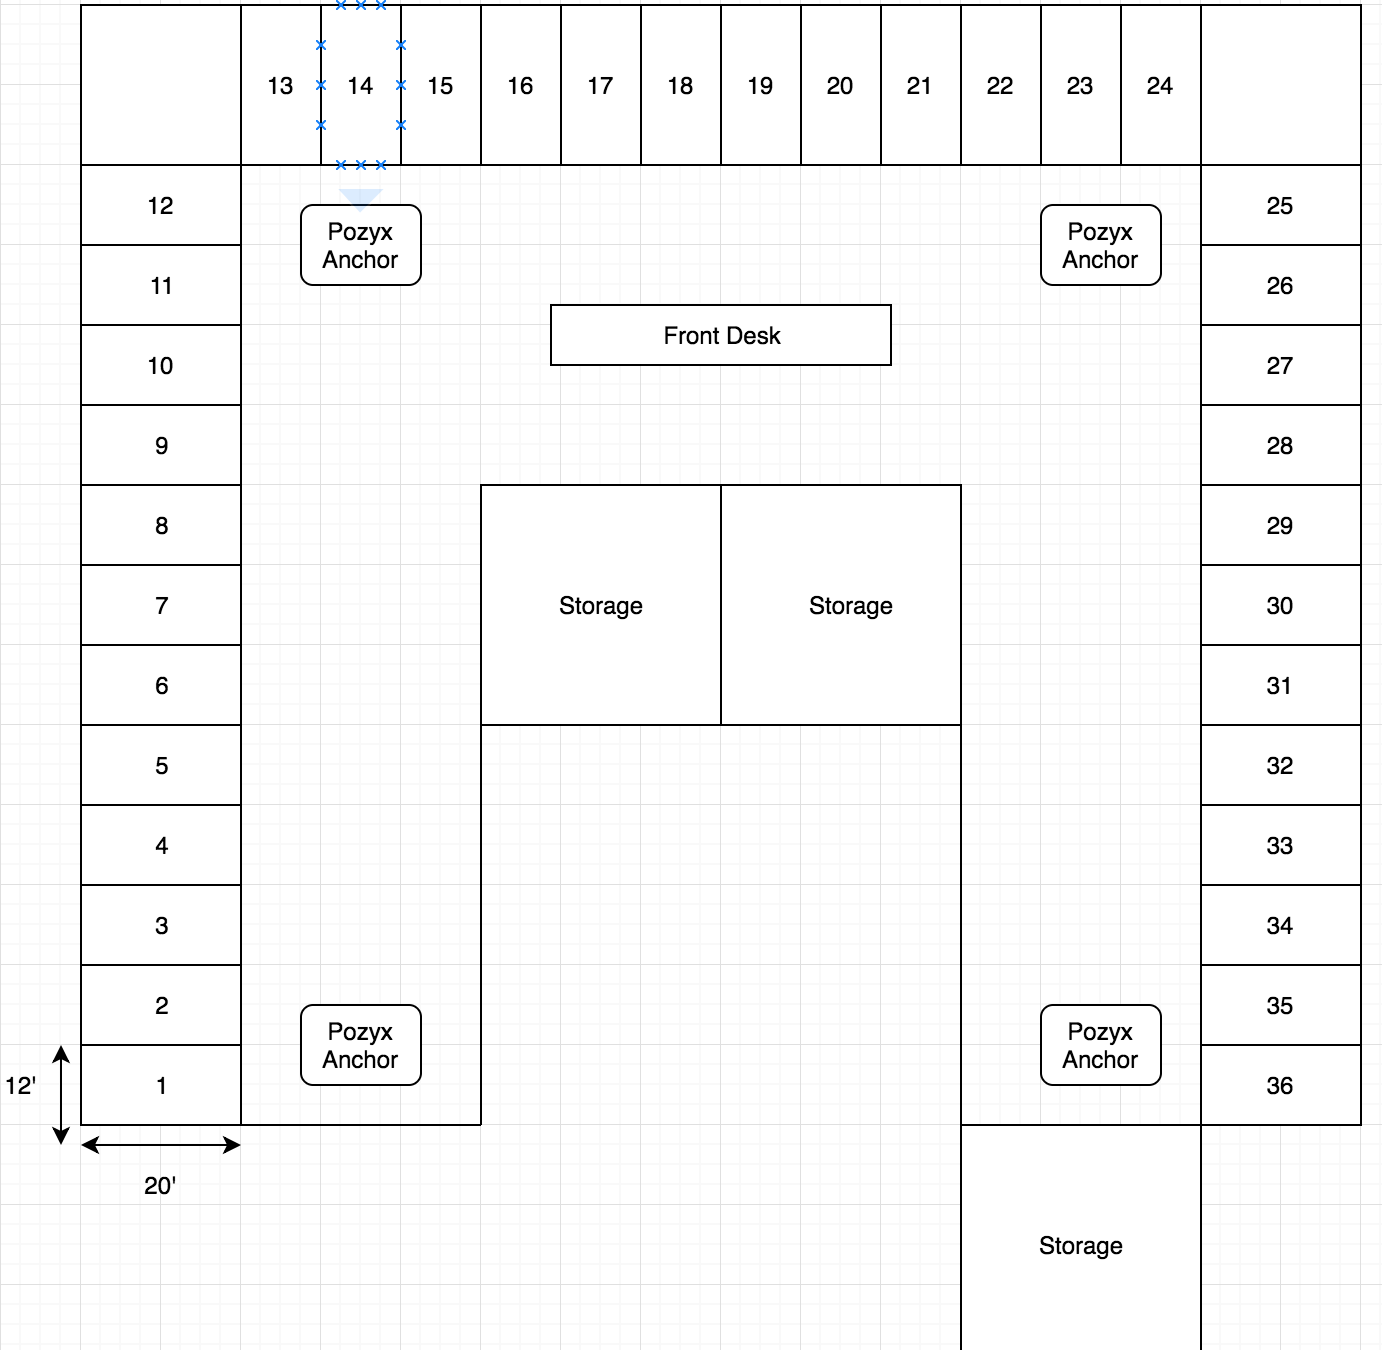
\includegraphics[scale=0.6]{np.png}\\
		\end{center}

\section{Weekly Updates}
	\subsection{Week 1 \& 2}
		\begin{itemize}
			\item 8/29/2017 Emailed group members and setup group message for effective
			communication.
			\item 8/29/2017: Me and my group members introduced ourselves in person and started a group message to conduct further communication for the rest of the project.
			\item 8/30/2017 The group’s first meet-up and decided on a time to meet WenZhan Song, 
			our new mentor. We chose 9/1/2017
			\item 9/1/2017 We met with our mentor. We discussed the project and proposed 
			solutions and necessary equipment for the project.
			\item 9/1/2017: We chose to meet up with our mentor today and discuss the project.  Due to a scheduling conflict I personally was not able to attend the meeting, but my other two group mates were an immediately filled me in.  Dr. Song said that we were to use him as a resource only when we run into problems throughout the duration of the project, but was willing to help by providing some initial ideas.  Since Children’s wants to be able to know what room a ventilator is in GPS is immediately not going to work due to accuracy.  To locate the ventilators he suggested that we use bluetooth or wireless internet signals to triangulate its position with hotspots in the hospital.  He also suggested that we use a raspberry pi and that we get some sort of enclosure for it as well.
			\item 9/7/2017 Emailed our client and decided to have a conference call 9/11/2017
			\item 9/7/2017: Today I constructed an email to my clients to ask what a good time to have a conference call would be.  We noted that we wanted to introduce ourselves and discuss some of the details of the project as well as how we would proceed.
			\item 9/11/2017 Client conference call today. We discussed many details regarding the 
			project and what exactly it is they wanted and how we would be able to do that. Also 
			discussed a time to meet and visit the hospital
			\item 9/11/2017: Today was our conference call with our client.  Unfortunately it is also monday in the middle of a hurricane so only Jocelyn was able to be on the phone call rather than all three members we contacted in the email.  As mentioned in the post about the email we begin by introducing ourselves and immediately began discussing the project and what it was they were looking for in detail.  They started by telling us how many ventilators they have and how many are usually in use.  She also mentioned that sometimes they have to rent ventilators when they don’t have enough so I made the note that we need to make the tracking device removable so that this can be added and removed from rented vents.  We also discussed our intention to wireless access points as “satellites” to triangulate the ventilators position with increased accuracy rather than GPS which was definitely news to her.  So when we asked if we would be able to have access to a map of where hospital access points were she said she would have to look into it.  Finally we discussed coming to the hospital to meet them in person and continue working on the project.
			\item 9/12/2017 Created a shared document of a draft of the group problem statement 
			created by me and edited by Alex and Brian. Decided on a final project statement and 
			turned it in.
			\item 9/12/2017: Today I created the problem statement for our group.  Using the details that were discussed on our earlier conference call with Jocelyn and the help from Dr. Song I were able to narrow down our problem statement.  This was then, of course, reviewed by my groupmates before we submitted it.
			\item 9/18/2017: We have scheduled a meeting with our clients for Thursday September 28, 2017.
		\end{itemize}

	\subsection{Week 3 \& 4}
		\begin{itemize}
			\item 9/21/2017: Emailed out clients, Dr. Kamat and Dr. Grunwell, about a time and date to meet.
			\item 9/22/2017: Today we finalized our meeting date through email with our clients to be Thursday September 29th, 2017 at 5:30 PM.
			\item 9/28/2017: Today I drove with my group members to visit the hospital and discuss the project as well as have dinner before we left to return to campus.
			\item 9/29/2017: The last thing we did this week was meet up to order a Raspberry PI, and further explore different ideas for our design now that we had plenty of information.
			\item This week we scheduled a visit in person with our client at Children’s Healthcare of Atlanta at Egleston. We met to get a firsthand view of the ventilators and other hospital equipment that they would like to have monitored. We spoke with a nurse at the hospital to discuss what she wants exactly and what portions of the problem are most important to her and other employees. From her we want to generate the first “full” design of the project and finalize our budget and collect the necessary equipment.
		\end{itemize}
		
	\subsection{Week 5 \& 6}
		\begin{itemize}
			\item October 3rd, 2017 Alex created a google doc for the group to begin working on the midterm report.  The work was split rather evenly and I contributed to the background research and preliminary design portion of the report.  After completion and review this was submitted.
			\item October 3rd, 2017 I also created and initialized a private GitHub Repository for the group to create and version controlle code when we began developing the software. This was later deleted and re-created by Alex later on because of permission issues.
			\item October 4th, 2017 Alex created a google calendar to help organize and optimize or time working together.
			\item October 9th - 10th, 2017 Created an submitted a presentation for our midterm presentation on Wednesday.  I spent most of my time on the problem constraints, mentor and client feedback, as well as existing product.  Having completed the presentation Dr. Johnsen mentioned that across the board our contraints from our client were not well outlined.  I intend to fix this.  More on this in my notebook.
			\item October 12th, 2017 Began parsing an existing location project on GitHub using a raspberry pi to determine what we like about this project and what we do not.  Although this may help us with the portion of the project involving location much more will need to be added to determine machine state and display in a UI.
			\item This last week was all about gathering together and organizing what it is we have done so far and ironing out an exact plan about what we plan on doing for the rest of the semester in the effort of completing our project.  As a group the presentation did not go as well as planned in my opinion, but that does not change where we stand on the project, which I believe is better than we were able to present.  One last comment on the last project in feedback you mentioned that it was absurb that I claimed that the hours were 16.  I believe that i misunderstood the format.  I thought that it was supposed to be total hours up until the date the report was turned in.  That all meaning progress report two encompassed 8 hours not 16.  Sorry for the confusion.
		\end{itemize}
		
	\subsection{Week 7 \& 8}
		\begin{itemize}
			\item October 18th - 26th, 2017 Alex found a highly rated series of videos/tutorials on how to program in Swift.  Swift is a language used to develop application in iOS the operating system of all iPhones.  The iPhone application is what the clients requested to be the user interface and the software used to communicate with the raspberry pies. \href{https://www.youtube.com/watch?v=83WXmhin_LU}{Youtube Series}
			\item October 20th - 23rd, 2017 Powering the pie is the only part of this project I am currnetly up happy with.  Our clients did not want us to pull power from the equipment, which is the most integrated, permenant, and clean solution.  The bandaid to the problem is of course external batteries, which are ugly, unfinished, and consumable.  Instead, you could uses and much larger battery power supply in the neighborhood of 10,000 mAh that will last a long time and be rechargable. Thiw would look slightly better but nonetheless is still a hassle for the end user that does not need to be there.  Especially in the case of the nurses we spoke with who stressed many times that this has to help without adding any steps to there current way of using the equipment.  Some how the idea of locating equipment that now needs to be charged doesn't really do that.  I would like to reach out to the client and see if the limitation of integrating power is set in stone and if it is my final idea for now is solar.  A small panel on the outside of the enclosure that provides the low amps needed by the pie as well as a pie that is in an off state when it is obivous it wont be tracked.
			\item October 23rd, 2017 Alex began to look for enclosures for the raspberry pie.  The reason we have waited so long to do this is because of a couple requirements.  We wanted to first determine whether or not we would need an external switch on the enclosure for determining in-use/not-use state or a change in temperature from the equipment.  We decided on a switch after now starting for two reasons.  One the change in temperature method assumes that all equipment to be tracked have a large enough delta and there is the added sensor expense on every tracker.  This all to say we now know we need an enclosure that will incorperate a push-button.
			\item So far we have spent basically all of our time on the specifics of how to triangulate the 
			necessary hospital equipment and while we definitely have settled on a good idea it was time to shift our focus.  Both of my group members and I began to learn how to program in Swift from tutorial videos found by Alex.  I too watched these videos and spent some time in XCode practicing as well as translating our idea into software.  However another area that needs some attention is power.  Dr. Johnsen asked a good question during our presentation about how a battery is a fairly temporary answer to the problem.  However, being that our clients do not want us to pull power from the equipment itself we are left with a big problem.  Ontop of software I am spending time looking for a more convient and permenant solution to the power problem.
		\end{itemize}
		
	\subsection{Week 9 \& 10}
		\begin{itemize}
			\item November 1st, 2017 Finished watching the YouTube Series on how to use swift and implemebering different example to practice with.
			\item November 4th, 2017 Today we officially started the software development as a group in XCode.  As far as the GUI goes things are looking fairly simple.  Our goal is to superimpose the tracked positions on to a map of the main wing of the Hospital and if we can have live tracking of this equipment rather then just a refresh every few seconds or minutes.  On the tracking side of the code it is starting to look more diificult then we were expecting.  The idea of wifi and bluetooth tracking is more complex then we had thought and it is looking like it will be more accurate then GPS, but it will still have an error radius of 2.5-5 meters which in the hospital could easily be the difference between rooms.
			\item November 7th, 2017 Today Alex found a kit that could be imported to display the Map of the Hospital that would be the main if not only page of our app at the moment.
			\item November 10th, 2017 Running in to many issues with developing our own set of algorithms we are continuing to look elsewhere to see how others have tackled the issue and if there is anything effective we could build off of.  This has led us to Node.js.  They are using a longer list of hardware then we are including some developed in house by them, but a lot of there work focused on the software and there are some promising leads.
			\item After all the time we have spent researching promising methods for this project in the first half of the semester we have begun to realize that the largest hurdle of the project will be in the software development.  A lot of different groups have tried it and not many that we have found have had total success.  The battle for us will be accuracy versus power consumption since our clients need mobility and dont want us piggy backing power from their equipment.  Having begun the development process we are finding that bluetooth is lacking the range and wifi in to inaccurate for the size of the hospital room.  The following weeks will involve some more research into others groups work and solutions to this problem and further software development.
		\end{itemize}
		
	\subsection{Week 11 \& 12}
		\begin{itemize}
			\item November 15th, 2017 After talking with Alex, today was all about finding a way to increase the range of bluetooth for bluetooth triangulation or increasing the accuracy of the wifi traingulation.  I did not have high hopes for this because the traditional way to increase accuracy in triangulation is increasing the number of "satellites" or in our case access points around the hospital which are very limited in numbers.
			\item November 15th, 2017 In our research Alex found a project called pozyx.  They have been able to construct harware that has a larger range then bluetooth and increased accuracy compared to both of them with regards to indoor location tracking.  This is exactly the problems we have been having and need to solve.  They do not provide much in the way of software and we would still need to indegrate what they do bring into our app for our particular purposes, but this harware would allow us to have accuracy far beyond what we anticipated and could even implement it such that it will live track there equipment as it is being moved around.
			\item November 15th, 2017 Having determined that we would not be able to go on creating out work from scratch and having found help from the pozyx project we needed to re-work our plan and budget.  Me and Alex did this together and decided that we would still need to raspberry pi from our initial proposal but would like to add some anchors to complete this new plan.
			\item November 28th, 2017 Began working on the groups final report and presentation for the end of the semester, outlining what has changed and where we stand.
			\item November 29th, 2017 As a group we constructed and email with the people from pozyx discussing the project and our goals looking for some insight and aid.
			\item November 29th, 2017 Spent time working on the project with Alex and Brian for a significant amount of time trying to finalize as much as possible as finals are coming up and free time will be at a premium.
			\item What I pressume will be our greatest failure while working on this project was assuming that we would be able to develop the software from the ground up with little to no help from elsewhere.  This led to many issues and paths that took up a lot of our time and woud not work.  We have brought them up many times in these progress reports.  We thought that we would have a prototype completed in time to begin optimizing power consumption and finding a cleaner and lower maintaince solution then batteries, but have instend spent most of our time trying to find a method of indoor location that will even be accurate enough to locate equipment down to a room and floor in a consistantly reliable way.  While we now believe we have a solution I do wish we had found this earlier in a our research process as it could have saved us a lot of time and trouble and we could be further ahead today.
		\end{itemize}

	\subsection{Week 13 \& 14}
		\begin{itemize}
			\item January 8th, 2018 Alex began emailing and updating our mentor with the status of our project and new short and ling term goals.  Of course keeping Brian and I in the loop the entire time.
			\item January 9th, 2018 I began to email Roger Hilton to discuss a change in the alotted budget for our group so we could begin the process of ordering the new hardware.
			\item January 10th, 2018 Alex and Brian met up with Dr. Wen Zhen Song to discuss the project face to face just to make sure we are on the right trajectory for the semester before we start to move forward.
			\item January 22nd, 2018 Roger Hilton has granted our budget increase and I am filling out another form for him including the list of hardware from Poyzx and the pi without the developer kit this time.
			\item January 26th, 2018 Items list has been completed and sent to Roger Hilton to be ordered and we now turn our focus to continuing development on the iOS app while we wait for the hardware.
			\item This week was all about getting back on track after our long holiday break. The first thing that I needed to do for the group was email Roger Hilton to ask about a budget adjustment. The last few things that we did last semester was determine that bluetooth and WiFi triangulation would not work for our needs and this meant we need an entirely new solution. THis landed us on UltraWideBand technology, which shares the benefits of both Bluetooth and WiFi. This of course means that we would need new hardware, which led to a massive change in the needed budget.  Alex and Brian started the semester by updating and touching base with our mentor Dr. Wen Zhen Song while i worked out the budget and list of required hardware for the new design.
		\end{itemize}
		
	\subsection{Week 15 \& 16}
		\begin{itemize}
			\item January 30th, 2018 - February 8th, 2018 The last two weeks we have been waiting on hardware so we turned all of our combined focuses on the GUI for our project. We need to have a GUI for iOS as our clients requested so that all the nurses, doctors, and other hospital staff can use the in door tracking. We spent the last two weeks laying out the layers and frames required. We are includeing a map with pinpoints for each and every tracked device and more device details if clicked. We also are including a page with a list of all the devices currently being tracked.  We need to contact our clients to ask for there map resource elements that they use on their app for the visitors.
			\item Febraury 9th, 2018 Today we got an email that most of our hardware have arrived all we are waiting for now is the equipment that comes with the Poyzx development kit.
			\item This week was all about the app development and the software on the front and back end. Waiting on the hardware this week ended up being a good thing so we could catch up on the work that needed and needs to be done on the tracking and information in the application.
		\end{itemize}
		
	\subsection{Week 17 \& 18}
		\begin{itemize}
			\item February 13th, 2018 We finally are expecting our hardware to arrive this week so as a group we met up and started to restructured out github repository. We initially had many programs and a large amount of code from last semester when we tried to use bluetooth to track the pi and we need to switch over to include the pozyx and arduino libraries and transfer what we have to work with our new hardware and UltraBand Technology tracking.
			\item February 19th, 2018 The harware finally arrived. I personally picked up the Pozyx Development Kit and I took out the tracking chips and started initialzing the shields with my arduinos. It took a while for these to ship form the UK so we lost some time and need to catch back up.
			\item February 20th, 2018 Today we setup the four anchors in Alex's room and started writing the code in the Arduino IDE with the help of the Pozyx documentation site and the example programs. Four of the five shields were calibrated correctly from yesterday and we had to re calibrate the fourth.  Not using the anchors and just running our code to test the range between the two shields we were seeing result even better then expected for this hardware. Im sure that will degrade when we start localizing form the anchors but it is good news either way.
			\item February 21st, 2018 Today I moved into localization. Previously we were using the UltraBand Tech on the shields to have one act as a reciever and the other as a transmitter and test there range from each other using the LEDs on both Arduinos to light up for every 5cm more apart from each other. While its great for calibration and hardware testing and farmiliarizing ourselves with the hardware it is not our goal for the project. That is were localization comes in and in the test room we use four anchors or ICs that wont be moving and in a preciese location each to triangulate a shield the four measuring time of course. Results we ok we still need to improve the accuracy we are not seeing uncertainty that we were expecting and the sample rate is saturating, but we are tracking finally in real time.
			\item February 22nd, 2018 Today we met up as a group to again turn our focus back to software. We have been waiting for this hardware so long that we were worried about the missed time, but we had a lot of success and decided we need to focus on the app. We need to store data and overlay on GUI map of the hospital.
			\item This week we finally collected our hardware and so for the past two weeks that was our entire focus. We made progress though and have started the localization of the shields. Hopefully in the coming weeks we will be able to finish and tweek that so that all that is left to do is the app making all the hardware more presentable.
		\end{itemize}
		
	\subsection{Week 19 \& 20}
		\begin{itemize}
			\item March 21st, 2018 We have completed the process of uploading data to our google cloud so that the positioning and timing data can be retrieved by the application.
			\item March 23rd, 2018 Worked on designing a case for the raspberry pi zero W, pozyx shield, and power supply so what will be attched to the various hospital equipment will be just one small unit.
			\item March 23rd - 30th, 2018 We spent most of our time since spring break working on\/developing the application as it is the final major milestone before we can put our whole project together. Focused on keeping the page depth and parallels as small as possible with location and equipment details. We are connected it to the DB with all the location data and preparing to calibrate for demonstration.
			\item March 25th-27th, 2018 Various work on the final connections of everything that we need in the final unit. Included removing default GPIO pins and soldering in on the required pins a specified length and trying to keep everything as neat exchangable and clean as possible. 
			\item These last two weeks have been about application development, database management, data transfer, and putting on the hardware together in a small neat package. We are still working on the application and design for an enclosure for everything in one unit, which will lead to final calibrating, testing, \& debugging.
		\end{itemize}
		
	\subsection{Week 21 \& 22}
		\begin{itemize}
			\item March 31st, 2018 Alex continued work on the iOS application and focused on the splash screen and the tracking tab. The focus is all on finishing the tracking tab such that the position data is working for all of our reciever units and calibrating them. This leaves the final task for the app of getting the transmitter, reciever, and apllication all to communicate through our database.
			\item April 5th, 2018 Started work on the abstract for our upcoming showcase.
			\item April 8th, 2018 Compeleted the work on the case design for the transmitters, now just to manufacture.
			\item April 10th, 2018 Started work on the groups final report and poster for the completion of the year long capstone project and continued work on the abstract.
			\item April 12th, 2018 Today we completed work on the abstract and I transferred the information to a more clean and professional format.
			\item Everything in the project is comming together. We are definitely on schedule, but still have plenty of work to do to make sure that all of these components work together and everything is in a complete and presentable clean looking package for the showcase. On top of all the project work we needed to start allocating time to work on the presentation side of the showcase with out abstract report and poster as well.
		\end{itemize}

	\paragraph*{}
		\textbf{Total Time Spent: } 110

\section{Final Product}
	\paragraph*{}
		Indoor tracking is cutting-edge technology, and the topic is still being researched, refined, and developed every day. Our group was tasked with designing a portable tracking device along with an application to track ventilators and respirators in a specific wing of the hospital at Children’s Healthcare of Atlanta at Egleston, with the intent to scale. Along with the location tracking, CHOA had further requirements: an in-use detection system and maintenance data to prevent downtime. Our system is made up of a Raspberry Pi in tandom with Pozyx ultra-wideband indoor tracking technology to implement location tracking with 1 - 5cm error radius; an iOS application was built for the hospital staff to easily view the tracking system. The transmitter unit uploads data through the Raspberry Pi using a Python script to a Google Cloud containing a MySQL server, which is accessed/displayed by our iOS application. A button on the device is used to indicate if a ventilator is being used or not along with a corresponding LED on board. We were required to make the transmitter wireless and removable yet, unable to integrate our tracking device with the equipment; the corresponding trade off is rechargable power. We could not use the hospital wing for testing, so we used a diagram of the room that we set the system up in as a replacement as a proof of concept. To fully implement within the hospital wing would simply require updating the appropriate location of the Pozyx anchors in the Python script, connecting the Raspberry Pi to the hospital’s network, and authorizing the hospital’s IP address in our Google Cloud instance. We included a maintenance date and time counter in the database for each tracker ID which can be accessed and managed through the application. To finalize our design, we transferred our implementation from a Raspberry Pi 3 to a Raspberry Pi Zero for size and cost and enclosed the entire tramitter unit in an enclosure to allow for a more-compact tracking device.

\section{Source Code}
	\subsection{Raspberry Pi 3}
		\begin{Verbatim}[fontsize=\small]
import os
import datetime
import time
from time import sleep
from firebase import firebase
import RPi.GPIO as GPIO
GPIO.setmode(GPIO.BCM)
GPIO.setwarnings(False)
from pypozyx import (POZYX_POS_ALG_UWB_ONLY, POZYX_3D, Coordinates, 
	POZYX_SUCCESS, POZYX_ANCHOR_SEL_AUTO, DeviceCoordinates,
	PozyxSerial, get_first_pozyx_serial_port, SingleRegister,
	DeviceList)
from pythonosc.udp_client import SimpleUDPClient
		\end{Verbatim}

		\begin{Verbatim}[fontsize=\small]
onLEDPin = 23
offLEDPin = 18
buttonPin = 17
GPIO.setup(onLEDPin, GPIO.OUT)
GPIO.setup(offLEDPin, GPIO.OUT)
GPIO.setup(buttonPin, GPIO.IN, pull_up_down = GPIO.PUD_UP)
GPIO.output(offLEDPin, GPIO.HIGH)
GPIO.output(onLEDPin, GPIO.LOW)
		\end{Verbatim}

		\begin{Verbatim}[fontsize=\small]
def format_time():
    dTime = datetime.datetime.now().strftime('%Y-%m-%d %H:%M:%S')
    return dTime

def in_use():
    global inUse
    if (inUse == 0):
        inUse = 1
        GPIO.output(offLEDPin, GPIO.LOW)
        GPIO.output(onLEDPin, GPIO.HIGH)
    else:
        inUse = 0
        GPIO.output(offLEDPin, GPIO.HIGH)
        GPIO.output(onLEDPin, GPIO.LOW)
		\end{Verbatim}

	\subsection{Pozyx Anchors}
		\begin{Verbatim}[fontsize=\small]
pozyx = PozyxSerial(serial_port)
    r = ReadyToLocalize(pozyx, osc_udp_client, anchors,
    	algorithm, dimension, height, remote_id)
    r.setup()
    while 1:
        r.loop()
        if not GPIO.input(buttonPin):
            in_use()
        maintenance = format_time()
        data = {"ID": Id, "X": x, "Y": y,
        	"InUse": inUse, "Maintenance": maintenance}
        firebase.post('/Ventilator', data)
        time.sleep(5)
		\end{Verbatim}

	\subsection{Firebase Database}
		\begin{Verbatim}[fontsize=\small]
var ref:FIRDatabaseReference?
var databaseHandle:FIRDatabaseHandle?
fileprivate var chart: Chart?
var currentX, currentY: Double
var inUse: Bool
var xStack = DoubleStack()
var yStack = DoubleStack()
		\end{Verbatim}

		\begin{Verbatim}[fontsize=\small]
databaseHandle = ref?.child(``X'').observe(.childAdded, with: { (snapshot)
	self.xStack.push(snapshot.)
	self.currentX = self.xStack.pop()
	createGraph()
})

databaseHandle = ref?.child(``Y'').observe(.childAdded, with: { (snapshot)
	self.yStack.push(snapshot.)
	self.currentY = self.yStack.pop()
	createGraph()
})
		\end{Verbatim}

	\subsection{Application}
		\begin{Verbatim}[fontsize=\small]
import SwiftCharts
		\end{Verbatim}

		\begin{Verbatim}[fontsize=\small]
let chartPoints: [ChartPoint] = [(currentX, currentY)].map{
	ChartPoint(x: ChartAxisValueInt($0.0), y: ChartAxisValueInt($0.1))}
		\end{Verbatim}

		\begin{Verbatim}[fontsize=\small]
let xModel = ChartAxisModel(firstModelValue: 0, lastModelValue: 10,
	axisTitleLabels: [ChartAxisLabel(text: "", settings: labelSettings)],
	axisValuesGenerator: xGenerator, labelsGenerator: labelsGenerator)
    
let yModel = ChartAxisModel(firstModelValue: 0, lastModelValue: 10,
	axisTitleLabels: [ChartAxisLabel(text: "",
	settings: labelSettings.defaultVertical())],
	axisValuesGenerator: generator, labelsGenerator: labelsGenerator)
		\end{Verbatim}

		\begin{Verbatim}[fontsize=\small]
let chart = Chart(
    frame: chartFrame,
    innerFrame: innerFrame,
    settings: chartSettings,
    layers: [
        xAxisLayer,
        yAxisLayer,
        guidelinesLayer,
        chartPointsLayer
    ])
		\end{Verbatim}

\newpage
\section*{Appendices}
	\begin{figure}[!htb]
		\centering
		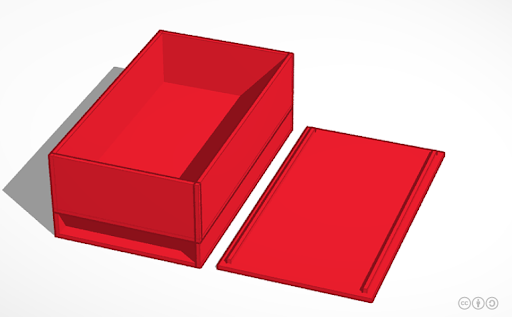
\includegraphics[scale = .75]{Enclosure.png}
		\caption{Tinkercad 3D Enclosure}
	\end{figure}

	\begin{figure}[!htb]
		\centering
		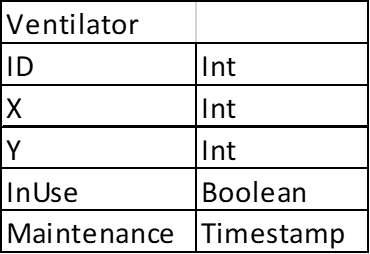
\includegraphics[scale = .75]{DatabaseTable.png}
		\caption{Database Table}
	\end{figure}

	\begin{figure}[!htb]
		\centering
		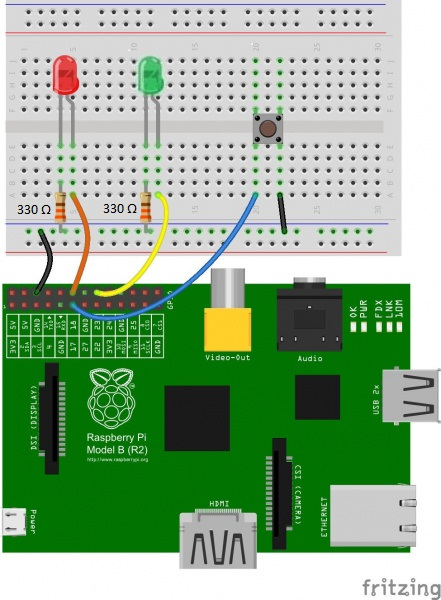
\includegraphics[scale = .5]{GPIOCircuit.jpg}
		\caption{Raspberry Pi 3 GPIO Circuit}
	\end{figure}

	\begin{figure}[!htb]
		\centering
		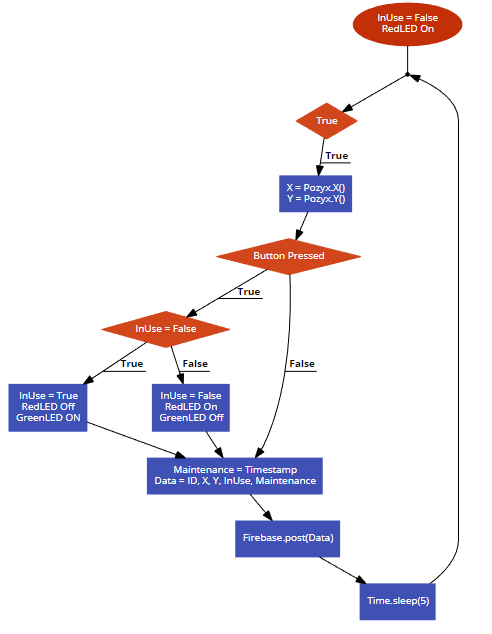
\includegraphics[scale = .75]{PythonFlowchart.PNG}
		\caption{Python Script Flowchart}
	\end{figure}

	\begin{figure}[!htb]
		\centering
		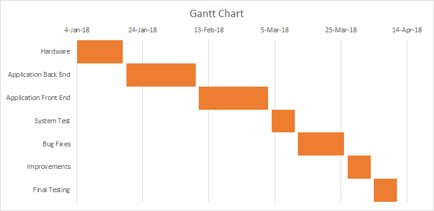
\includegraphics[scale = 1.3]{Gantt.jpg}
		\caption{Gantt Chart}
	\end{figure}

	\begin{figure}[!htb]
		\centering
		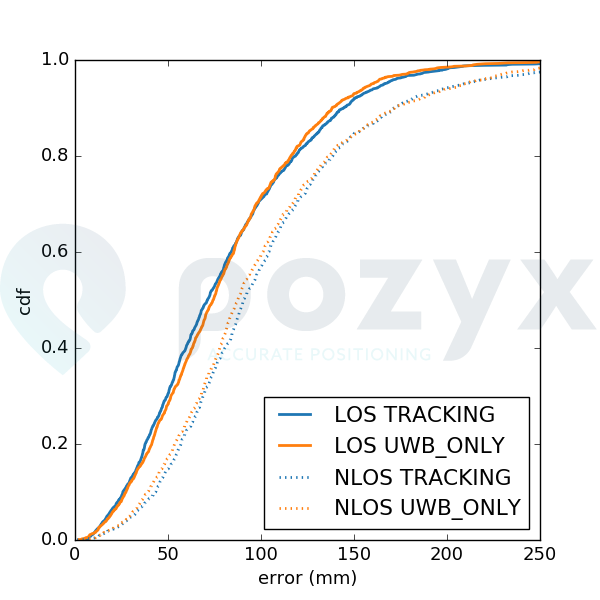
\includegraphics[scale = .4]{PositioningError.png}
		\caption{Pozyx Experimentally Measured Positioning Error in XY Plane}
	\end{figure}

	\begin{figure}[!htb]
		\centering
		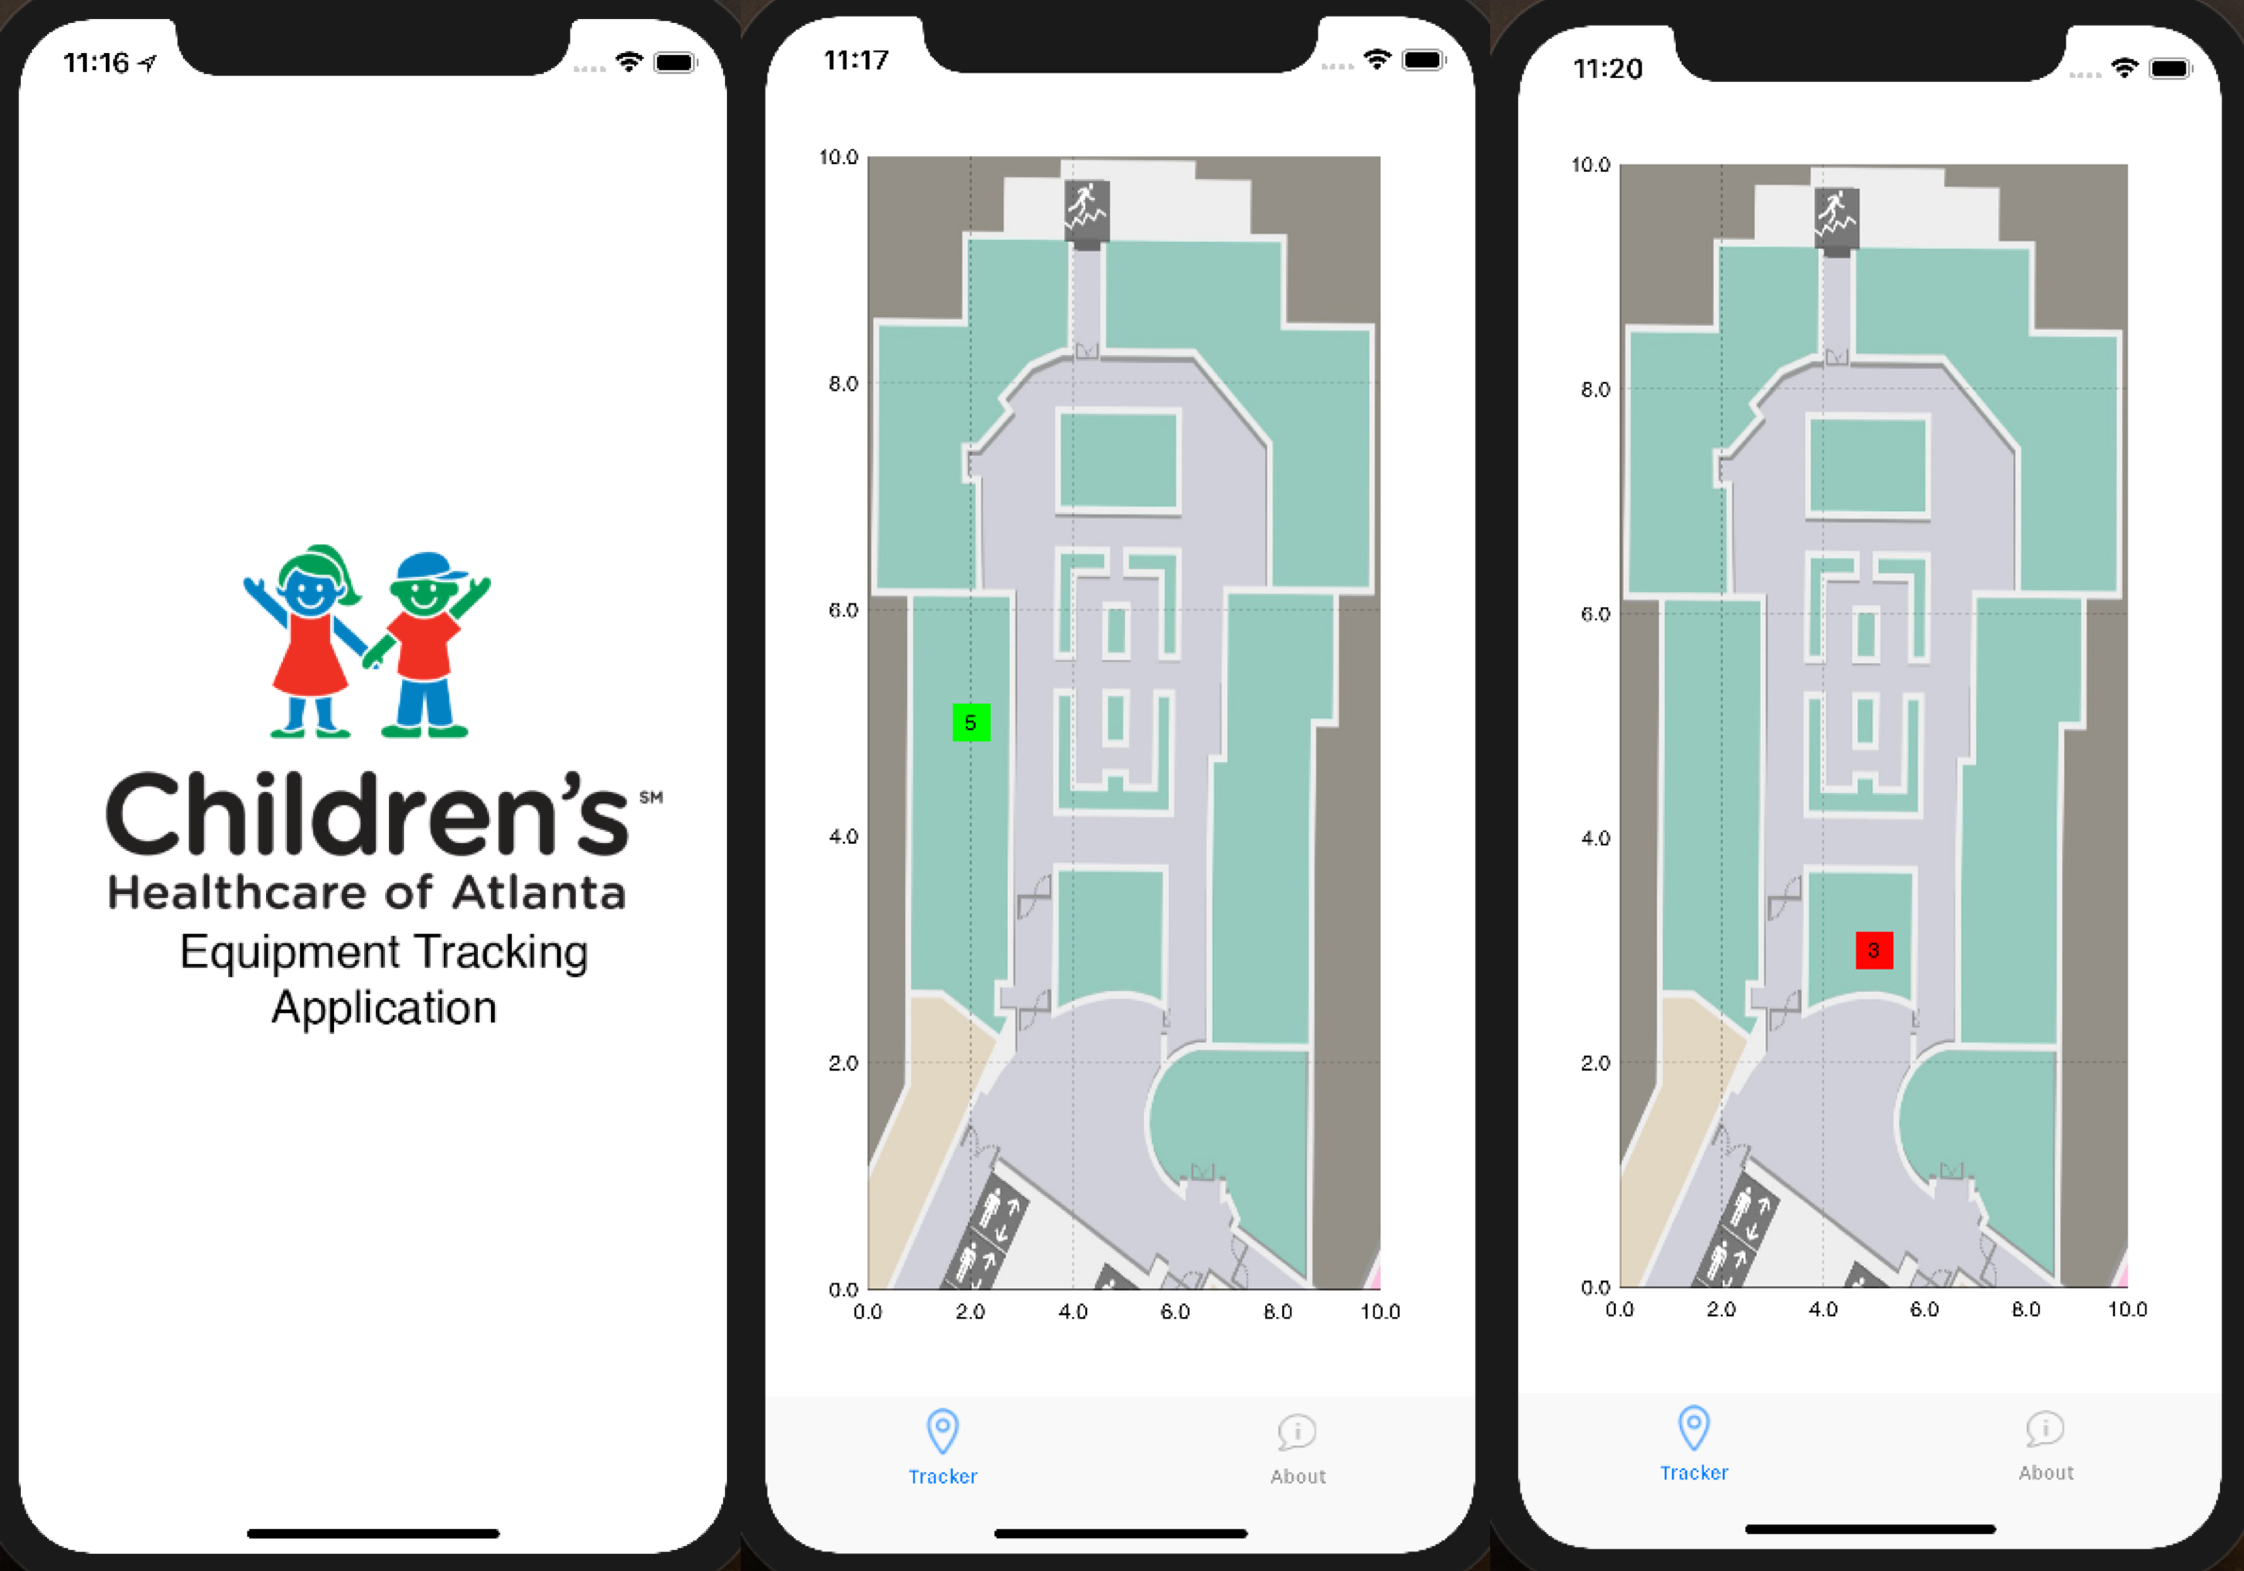
\includegraphics[scale = .45]{iOSApp.png}
		\caption{iOS Application}
	\end{figure}

\end{document}